
\subsection{Calibration changes the composition regime}
Raw addition of independently trained logits performs poorly, especially for three-way conjunctions. After scalar calibration, several soft AND rules converge to similar quality. We use the log-probability product because it is simple, compositional, and needs no conjunction-specific model.

\begin{table}[t]
\centering
\caption{Composition of independently learned predicates in the mechanism study.}
\label{tab:composition}
\small
\begin{tabular}{lcc}
\toprule
Rule & 2-way F1 & 3-way F1\\
\midrule
Raw logit add & 0.7148 & 0.5633\\
Min calibrated logit & 0.8140 & 0.7428\\
Log-probability product & \textbf{0.8142} & 0.7459\\
Soft-min ($\tau=1$) & 0.8141 & 0.7451\\
Correlation weighted & 0.8142 & \textbf{0.7470}\\
\bottomrule
\end{tabular}
\end{table}

\begin{figure}[t]
\centering
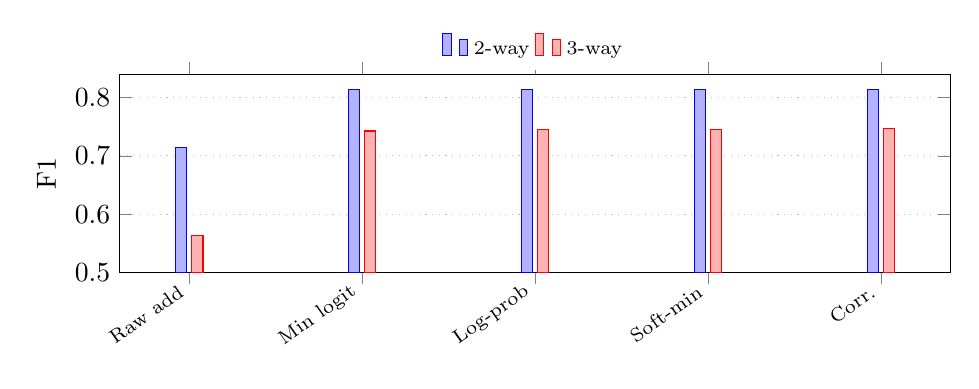
\begin{tikzpicture}
\begin{axis}[
  width=\columnwidth,height=4.1cm,
  ybar, ymin=0.5,ymax=0.84,
  ylabel={F1},
  symbolic x coords={Raw,Min,LogP,Soft,Corr}, xtick=data,
  xticklabels={Raw add,Min logit,Log-prob,Soft-min,Corr.},
  x tick label style={rotate=35,anchor=east,font=\scriptsize},
  legend style={font=\scriptsize,draw=none,at={(0.5,1.02)},anchor=south,legend columns=2},
  ymajorgrids=true, grid style={dotted}, bar width=4pt,
]
\addplot coordinates {(Raw,0.7148) (Min,0.8140) (LogP,0.8142) (Soft,0.8141) (Corr,0.8142)};
\addplot coordinates {(Raw,0.5633) (Min,0.7428) (LogP,0.7459) (Soft,0.7451) (Corr,0.7470)};
\legend{2-way,3-way}
\end{axis}
\end{tikzpicture}
\caption{Calibration, rather than a complex combination rule, drives the improvement in semantic conjunction.}
\label{fig:composition}
\end{figure}

The earlier geometric formulation obtained 0.639 F1 for two-way soft AND and 0.476 for three-way literal boxes. The calibrated program algebra reaches about 0.814 and 0.746--0.747. We therefore retain calibration and the simple product rule in all later supervised methods; the novelty claim is the compiled execution representation, not the probability product itself.

\subsection{Cross-modal predicate quality}
The main benchmark is deliberately cross-modal: CLIP sees images, whereas every search-side method sees only MiniLM title embeddings. Table~\ref{tab:predicate_finalists} reports predicate quality and storage. The FP32 linear head reaches 0.745 mean F1. PQ64 preserves most of this at 0.737. Binary1-LS2 with int4 predicate weights reaches 0.721, ahead of the sparse low-bit variants while using the smallest program among the high-performing supervised methods.

\begin{table*}[t]
\centering
\caption{Cross-modal predicate quality averaged over three strict splits, with packed storage accounting. Program bytes are approximate serialized state per concept.}
\label{tab:predicate_finalists}
\small
\begin{tabular}{lrrrr}
\toprule
Method & Item B & Program B/concept & Mean F1 & Mean AP\\
\midrule
FP32 linear & 1536 & 1548 & \textbf{.745} & \textbf{.805}\\
PQ64 compiled linear & 64 & 65548 & .737 & .794\\
Binary1-LS2, FP32 weights & 56 & 1556 & .721 & .771\\
Binary1-LS2, int4 weights & \textbf{56} & \textbf{216} & .721 & .770\\
RSA4 sparse LUT & 192 & 3652 & .707 & .758\\
RSA2 sparse LUT & 96 & 580 & .702 & .747\\
RSA1 centered random & 48 & 292 & .688 & .723\\
RSA1 centered identity & 48 & 292 & .687 & .724\\
Zero-shot prompt difference & 1536 & 1536 & .604 & .565\\
Zero-shot concept name & 1536 & 1536 & .575 & .469\\
\bottomrule
\end{tabular}
\end{table*}

Two ablations are especially informative. First, int4 predicate quantization is nearly free: Binary1-LS2 changes from 0.72106 to 0.72053 mean F1 and from 0.77092 to 0.76973 AP when the semantic weight vector is quantized from FP32 to int4. Second, random rotation is not doing much at one bit: centered identity and centered random sparse programs obtain 0.6866 and 0.6875 mean F1 respectively. The final benchmark therefore does not support random rotation as the source of the strongest compact result.

The gap to the image teacher is not purely a quantization effect. Even the uncompressed FP32 MiniLM-side linear proxy is imperfect against image-defined semantics, so the oracle includes information that may simply be absent from product titles.
